\chapter{Motivation}

% Why I did this.

\section{The Standard Model}
\label{sec:sm}

The Standard Model (SM) of particle physics describes the physical properties and dynamics of fermions, the fundamental constituents of matter, and their interactions in the language of a Lorentz-invariant quantum field theory (QFT).
The Standard Model consists of a set of fermion fields, shown in Table~\ref{tab:fermions} and the local gauge symmetry group that acts on them
\begin{equation}
  G_{\text{SM}} = \suthree \times \sutwo \times \uone,
\end{equation}
which is composed of the subgroups
\begin{align}
  G_{\text{QCD}} & = \suthree \qquad \text{and} \nonumber \\
  G_{\text{EWK}} & = \sutwo \times \uone,
\end{align}
corresponding to the strong and electroweak interactions, respectively.
Each fermion field exists in a unique representation of $G_{\text{SM}}$, also summarized in Table~\ref{tab:fermions}.
The possible represenations of \suthree\ are triplet, conjugate, and singlet, denoted by $\mathbf{3}$, $\mathbf{\bar{3}}$, and $\mathbf{1}$, respectively, while the possible representations of \sutwo\ are doublet and singlet, denoted by $\mathbf{2}$ and $\mathbf{1}$, respectively.
All fermions exist in the singlet representation of \uone, only distinguished by differing values of the weak hypercharge $Y$.
Conversely, all fermions in non-singlet representations of \suthree\ and \sutwo\ have the same interaction strength, a feature known as universality.

\begin{table}[htbp]
\centering
\caption{
  The categories of SM fermions and the action of the SM local gauge symmetry group $G_{\text{SM}}$.
  Each category contains three members, one for each generation of the Standard Model.
  A corresponding table exists for the charge conjugated fields representing the anti-fermions.
  The subscripts $L$ and $R$ denote whether the field is left- or right-handed.
}
\label{tab:fermions}
\begin{tabular}{ l|c|c|c|c }
  Name & Symbol & $Y$ & \sutwo\ rep. & \suthree\ rep. \\
  \hline
  \hline
  Left-handed quark & $q_L$ & $\sfrac{1}{6}$ & \textbf{2} & \textbf{3} \\
  Right-handed up-type quark & $u_R$ & $\sfrac{2}{3}$ & \textbf{1} & \textbf{3} \\
  Right-handed down-type quark & $d_R$ & $\sfrac{-1}{3}$ & \textbf{1} & \textbf{3} \\
  \hline
  Left-handed lepton & $\ell_L$ & $\sfrac{-1}{2}$ & \textbf{2} & \textbf{1} \\
  Right-handed charged lepton & $e_R$ & -1 & \textbf{1} & \textbf{1} \\
  Right-handed neutrino & $\nu_R$ & $\sfrac{1}{6}$ & \textbf{1} & \textbf{1} \\
\end{tabular}
\end{table}

For each category of fermion listed in Table~\ref{tab:fermions}, there exist three generations or copies in the Standard Model, identical except for differing masses.
The lepton electroweak doublets contain the left-handed charged leptons and neutrinos
\begin{equation}
  \ell_{L} = \begin{pmatrix} \nu_e \\ e^-_L \end{pmatrix} ,
              \begin{pmatrix} \nu_\mu \\ \mu^-_L \end{pmatrix} ,
              \begin{pmatrix} \nu_\tau \\ \tau^-_L \end{pmatrix} ,
\end{equation}
and the right-handed lepton singlets contain the right-handed projections of the same leptons and neutrinos.
The quark electroweak doublets contain the left-handed up-type and down-type quarks
\begin{equation}
  q_{L} = \begin{pmatrix} u_L \\ d_L \end{pmatrix} ,
           \begin{pmatrix} c_L \\ s_L \end{pmatrix} ,
           \begin{pmatrix} t_L \\ b_L \end{pmatrix} ,
\end{equation}
and the right-handed quark singlets contain the right-handed projections of the same quarks.
% where $d'$, $s'$, and $b'$ are the electroweak eigenstates of the down-type quarks (further explained in Section~\ref{subsec:ewk}).
Quarks also exist in a strong triplet, which will be denoted with a superscript $c$ as necessary.

\subsection{Strong Interactions}
\label{subsec:qcd}

The strong interactions of quarks and gluons are described by quantum chromodynamics (QCD), with the Lagrangian
\begin{equation}
  \label{eqn:lqcd}
  \mathcal{L}_{\text{QCD}} = i \bar q_f^a \slashed D^{ab} q_f^b + m_f \bar q_f^a q_f^a - \frac{1}{4} G_{\mu\nu}^a G^{a,\mu\nu} + \theta \frac{g_s^2}{72\pi^2} \epsilon_{\mu\nu\rho\sigma} G^{c,\mu\nu} G^{c, \rho\sigma},
\end{equation}
where repeated indices are contracted.
The $q_f^a$ are the quark-field Dirac spinors of flavor $f \in \{u,d,c,s,t,b\}$, color $a \in \{r,g,b\}$ (the basis element of the triplet representation), and mass $m_f$.
The first term in Equation~\ref{eqn:lqcd} contains the QCD covariant derivative
\begin{equation}
  D_{\mu}^{ab} = \delta^{ab} \partial_\mu - i g_s \sum_{c} t_c^{ab} G_{c,\mu},
\end{equation}
where $g_s$ is the strong interaction coupling strength, $t_c$ are the eight $3\times3$ Hermitian traceless matrices that serve as the generators of the triplet representation of \suthree, and $G_c$ are the corresponding eight gluon fields.
The third term in Equation~\ref{eqn:lqcd} contains the gluon field strength tensors
\begin{equation}
  G_{\mu\nu}^a = \partial_\mu G_\nu^a - \partial_\nu G_\mu^a - g_s f^{abc} G_\mu^b G_\nu^C,
\end{equation}
where $f^{abc}$ are the structure constants of \suthree.
The non-Abelian structure of the \suthree\ group allows for 3-gluon and 4-gluon interactions in addition to the quark-antiquark-gluon interactions.

The last term in Equation~\ref{eqn:lqcd} violates CP conservation and produces a non-zero electric dipole moment (EDM) for the neutron.
Experimental limits onthe neutron EDM constraint the QCD vaccum angle $\theta$ to be smaller than $10^{-10}$.
The Peccei-Quinn theory provides a possible method to force $\theta$ to zero by introducing the hypothetical axion particle. The axion is a potential dark matter candidate and will be discussed further in Section~\ref{sec:dm}.

\subsection{Hadrons}
\label{sec:hadrons}

Free quarks and gluons are not observed in nature, only in bound states called hadrons.
This is a consequence of two factors: color confinement and aysmptotic freedom.

Color confinement is the hypothesis that colored objects are always confined to color singlet states and that no objects with non-zero color charge can propagate as free particles.
Thus, quarks can only exist in bound states of a quark-antiquark pair or three quarks, called mesons and baryons, respectively. 
Since gluons carry a color charge, they are confined to hadrons as well.
Confinement is a low-energy non-pertubative phenomenon, occuring only below the QCD confinement scale \lqcd. 
An analytic proof of color confinement does not exist currently; however, the running of the strong coupling constant $\alpha_s = \sfrac{g_s^2}{4\pi}$ provides a mechanism for it.

Due to higher-order corrections to propagators in a QFT, physical quantities such as coupling constants and masses acquire a scale-dependence, where the value of the quantity changes as a function of the probed energy scale $q^2$.
The process of recovering scale-invariance is called renormalization and ensures that any divergent terms from the higher-order corrections cancel out in the physical values.
Given the value of an arbitrary coupling constant $\alpha$ at some known scale $\mu^2$, the value of $\alpha$ at arbitrary scale $q^2$ is  
\begin{equation}
  \label{eqn:rge}
  \alpha (q^2) = \frac{\alpha(\mu^2)}{1 - \alpha(\mu^2) \left[ \Pi(q^2) - \Pi(\mu^2) \right]},
\end{equation}
where $\Pi(q^2)$ and $\Pi(\mu^2)$ are the self-energy correction of the propagator at scales $q^2$ and $\mu^2$.
While these individual terms are separately divergent, their difference is finite and calculable. 

For values of $q^2$ and $\mu^2$ larger than the confinement scale \lqcd, the difference between the gluon self-energy corrections to one-loop order is given by 
\begin{equation}
  \label{eqn:beta_qcd}
  \Pi_s(q^2) - \Pi_s(\mu^2) \approx - \frac{\beta}{4\pi} \ln \left( \dfrac{q^2}{\mu^2} \right)
\end{equation}
where $\beta$ depends on the number of quark and gluon loops.
For $N_c$ colors and $N_f$ quark flavors with mass below $\abs q$,
\begin{equation}
  \beta = \frac{11 N_c - 2 N_f}{12 \pi}. 
\end{equation}
In the Standard Model, $N_c = 3$ and $N_f \le 6$ regardless of energy, thus $\beta$ is always positive.
Combining Equations~\ref{eqn:rge} and~\ref{eqn:beta_qcd}, the evolution of $\alpha_s$ is given by
\begin{equation}
  \label{eqn:alpha_s}
  \alpha_s (q^2) = \frac{\alpha_s(\mu^2)}{1 + \beta \alpha_s (\mu^2) \ln \left( \dfrac{q^2}{\mu^2} \right)} \approx \frac{1}{\beta \ln \left( \dfrac{q^2}{\lqcd^2} \right)}
\end{equation}
for a sufficiently large energy scale $q^2 \gg \lqcd^2$.
Through electron-positron collisions, the value of $\alpha_s$ at the $Z$-pole has been measured to be $\alpha_s (m_Z^2) = 0.1181 \pm 0.0011$ with a corresponding confinement scale of $\lqcd = 218\MeV$.  

From Equation~\ref{eqn:alpha_s}, we see that $\alpha_s$ decreases with increasing $q^2$.
At $\abs q \sim 1\GeV$, the value of $\alpha_s$ is of $\mathcal{O}(1)$ confining quarks and gluons to hadrons in a strongly-bound non-perturbative state.
However, $\abs q \gtrsim 100\GeV$, we have $\alpha_s \approx 0.1$ which is small eneough that perturbation theory can be used and quarks can be treated as quasi-free particles.
This property of QCD is known as asymptotic freedom.

%\newpage
\subsection{Electroweak Interactions}
\label{subsec:ewk}

The electroweak interactions of fermions are described by $\sutwo \times \uone$ gauge group, with the Lagrangian
\begin{equation}
  \label{eqn:lewk}
  \mathcal{L}_{\text{EWK}} = i \bar \psi_i \slashed D \psi_i - \frac{1}{4} \vec W_{\mu\nu} \cdot \vec W^{\mu\nu} - \frac{1}{4} B_{\mu\nu} B^{\mu\nu}
\end{equation}
where repeated indices are contracted and $\psi \supseteq \{q_L, u_R, d_R, \ell_L, e_R, \nu_R\}$ is the set of SM fermions, and the gauge field tensors are given by
\begin{align}
  B_{\mu\nu} & = \partial_\mu B_\nu - \partial_\nu B_\mu \qquad \text{and} \nonumber \\
  \vec W_{\mu\nu} & = \partial_\mu \vec W_\nu - \partial_\nu \vec W_\mu + g \vec W^\mu \times \vec W^\nu ,
\end{align}
where $\vec W_\mu$ and $B_\mu$ are the gauge fields for \sutwo\ and \uone, respectively, and $g$ is the coupling strength for \sutwo.
The first term in Equation~\ref{eqn:lewk} contains the EWK covariant derivative
\begin{equation}
  D_{\mu} = \partial_\mu - i g \vec T \cdot \vec W_\mu - i g' Y B_\mu,
\end{equation}
where $g'$ is the coupling strength for \uone,
$Y$ is the \uone\ hypercharge of the fermion field,
and $\vec T$ are the generators of the doublet representation of \sutwo.
The generators can be written in terms of the Pauli spin matrices $\vec T = \vec \sigma / 2$ and only have non-zero action on left-handed particles. %  and right-handed antiparticles.
% and $\delta_L$ is 1 if the fermion field is left-handed and 0 if it is right-handed.
The values of the hypercharge $Y$ shown in Table~\ref{tab:fermions} are chosen such that the physical electric charge of each fermion is given by $Q =  T_3 + Y$.

Notice that Equation~\ref{eqn:lewk} does not contain a Dirac mass term like that found in Equation~\ref{eqn:lqcd}.
This is because the term
\begin{equation}
  m \bar \psi \psi = m \left( \bar \psi_L \psi_R + \bar \psi_R \psi_L \right)
\end{equation}
mixes the left-handed and right-handed fermions leading to a Lagrangian that is no longer invariant under \sutwo.
As the observed fermions are not massless, the Lagrangian given in Equation~\ref{eqn:lewk} is incomplete and an additional mechanism needs to be introduced to produce non-zero fermion masses.

\subsection{Electroweak Symmetry Breaking}
\label{subsec:ewsb}

Spontaneous electroweak symmetry breaking provides the mechanism we need, as well as providing masses to the weak gauge bosons. The \sutwo\ symmetry is broken by introducing a left-handed complex scalar doublet $\phi$ with $Y_\phi = \sfrac{1}{2}$ to the Lagrangian in the following manner
\begin{equation}
  \label{eqn:ewsb}
  \mathcal{L}_{\text{EWK}} \mapsto \mathcal{L}_{\text{EWK}} + \left|D_\mu \phi \right|^2 + \mu^2 \phi^2 - \lambda \left| \phi \right|^4 .
\end{equation}
We choose to write this complex doublet, known as the complex Higgs field, in terms of four real-valued fields so that
\begin{equation}
  \phi = \frac{1}{\sqrt{2}} \begin{pmatrix} \phi_1 + i \phi_2 \\ \phi_3 + i\phi_4 \end{pmatrix} .
\end{equation}
Fortunately, the two self-interaction terms create a Higgs potential with a degenerate global minimum at the vacuum expectation value (vev)
\begin{equation}
  v \equiv \langle | \phi | \rangle = \sqrt{ \frac{\mu^2}{\lambda}},
\end{equation}
and through gauge rotations we set $\langle \phi_{1,2,4} \rangle = 0$, removing three degrees of freedom and producing three massless Nambu-Goldstone bosons.
The remaining degree of freedom is the real Higgs field $H$ which expresses small peturbations around the vev in the third component of the complex Higgs field $\phi_3 = v + H$.

The kinetic term in Equation~\ref{eqn:ewsb} couples the complex Higgs field to the EWK gauge bosons as follows at the vev
\begin{equation}
  \left| D_\mu \phi \right|^2 = \frac{v^2}{8} \left[ \left(g W_\mu^1 \right)^2 + \left(g W_\mu^2 \right)^2 + \left(g' B_\mu - g W_\mu^3 \right)^2 \right].
\end{equation}
%\newpage 
Diagonalizing this term gives rise to the three massive weak bosons and the massless photon that we observe in nature:
\begin{equation}
  \begin{matrix}[l | l]
    W_\mu^{\pm} \equiv \frac{1}{\sqrt{2}} \left( W_\mu^1 \mp W_\mu^2 \right)
    & m_W = \frac{1}{2} vg \\
    Z_\mu \equiv \cos \thetaw W_\mu^3 - \sin \thetaw B_\mu
    & m_Z = \frac{1}{2} v \sqrt{g^2 + (g')^2} \\
    A_\mu \equiv \sin \thetaw W_\mu^3 + \cos \thetaw B_\mu
    & m_A = 0,
  \end{matrix}
\end{equation}
where $\tan \thetaw = g'/g$.
With this, we rewrite Equation~\ref{eqn:lewk} in terms of the observed electromagnetic, charged weaked, and neutral weak currents as follows:
\begin{align}
  \label{eqn:lewsb}
  \mathcal{L}_{\text{EWK}} % &= \mathcal{L}_{\text{EM}} + \mathcal{L}_{\text{CC}} + \mathcal{L}_{\text{NC}} \nonumber \\
  = \bar \psi_i \left( i \slashed \partial - e Q \slashed A \right) \psi_i
  & - \frac{g}{2\sqrt{2}} \bar \psi_i \left( T^+ \slashed W^+ + T^- \slashed W^- \right) \psi_i - \frac{1}{2} m_W^2 W_\mu^+ W^{-\mu} \nonumber \\
   & - \frac{g}{2 \cos \thetaw} \bar \psi_i (g_V - g_A \gamma^5) \slashed Z \psi_i - \frac{1}{2} m_Z^2 Z_\mu Z^\mu, 
\end{align}
where $e = g' \cos \thetaw$ is the charge of the electron, $T^\pm = (T_1 \mp i T_2)/\sqrt{2}$ are the weak isospin raising and lowering operators, and $g_V = T_3$ and $g_A = T_3 - 2 Q \sin^2 \thetaw$ are the vector and axial-vector couplings for the neutral weak current.

We can also expand Equation~\ref{eqn:ewsb} about the vev giving us the following Higgs Lagrangian
\begin{align}
  \mathcal{L}_H = \frac{1}{2} \partial_\mu H \partial^\mu H - \frac{1}{2} m_H^2 H^2
  & + \frac{m_H^2}{2 v} H^3 + \frac{2 m_W^2}{v} W_\mu^+ W^{-\mu} H + \frac{m_Z^2}{v} Z_\mu Z^\mu H \nonumber \\
  & + \frac{m_H^2}{8 v^2} H^4 + \frac{m_W^2}{v^2} W_\mu^+ W^{-\mu} H^2 + \frac{m_Z^2}{2v^2} Z_\mu Z^\mu H^2, 
\end{align}
where $m_H = \mu \sqrt{2} $.
Thus, we see that the real Higgs field $H$ has trilinear and quartic couplings to itself and the weak gauge bosons with coupling strengths proportional to the mass squared of the appropriate boson.
This suggests a way to introduce fermion masses through the Higgs field.

%\newpage
\subsection{Fermion Masses}
\label{subsec:yukawa}

Introducing Yukawa couplings between the complex Higgs field $\phi$ and the SM fermion fields enables us to add mass terms for the fermions.
First, we start with the terms for charged leptons,
\begin{equation}
  \label{eqn:lyuk}
  \mathcal{L}^{\text{leptons}}_{\text{Y}} = - \bar \ell_L Y_e \phi e_R - \bar e_R Y_e \phi^\dagger \ell_L,
\end{equation}
where $Y_e$ is the Yukawa matrix for the charged leptons.
In general, Yukawa matrices and thus mass matrices are non-diagonal and hence we need to convert from the electroweak eigenstates $f_{L,R}$ to the mass eigenstates $\tilde{f}_{L,R} = U^{f}_{L,R} f_{L,R}$ where $U^{f}_{L,R}$ is a unitary matrix.
With this we rewrite Equation~\ref{eqn:lyuk} in terms of the mass eigenstates
\begin{align}
  \mathcal{L}^{\text{leptons}}_{\text{Y}} & = - \bar{\tilde{\ell}}_{L} U^e_L Y_e \phi U^{e\dagger}_R \tilde{e}_{R} - \bar{\tilde{e}}_{R} U^e_R Y_e \phi^\dagger U^{e\dagger}_L \tilde{\ell}_{L} \nonumber \\
  & = - \bar{\tilde{\ell}}_{L} \tilde Y_e \phi \tilde{e}_{R} - \bar{\tilde{e}}_{R} \tilde Y_e^\dagger \phi^\dagger \tilde{\ell}_{L}, 
\end{align}
where $\tilde Y_e = U^e_L Y_e U^{e\dagger}_R$ is the diagonalized Yukawa matrix for the charged leptons.
After electroweak symmetry breaking, these terms become
\begin{align}
  \mathcal{L}^{\text{leptons}}_{\text{Y}} & = - \frac{v + H}{\sqrt{2}} \left( \bar{\tilde{e}}_L \tilde Y_e  \tilde{e}_R + \bar{\tilde{e}}_R \tilde Y_e^\dagger \tilde{e}_L \right) \nonumber \\
  & = - \left(1 + \frac{H}{v}\right) \left( \bar{\tilde{e}}_L \tilde M_e \tilde{e}_R + \bar{\tilde{e}}_R \tilde M_e^\dagger \tilde{e}_L \right) \nonumber \\
  & = - \tilde M_e \bar e e - \frac{\tilde M_e}{v} \bar e e H,
    \label{eqn:lmass}
\end{align}
where $\tilde M_e = v \tilde Y_e / \sqrt{2}$ is the diagonalized mass matrix for the charged leptons and $e$ is the set of massive Dirac spinors for the charged leptons.

From Equation~\ref{eqn:lmass}, we see that the Yukawa couplings between the complex Higgs field $\phi$ and the charged leptons result in a Dirac mass term and a coupling to the real Higgs field $H$ that is proportional to the mass of the charged leptons and the vev.
The same procedure is used to introduce mass terms for the down-type quarks whereas for the neutrinos and up-type quarks we must use the conjugate doublet $\phi_c = - i \sigma_2 \phi^*$ in place of $\phi$ to obtain the same result.

\subsection{Flavor Mixing}

For the charged leptons and up-type quarks, it is possible to define a basis of simultaneous electroweak and mass eigenstates, so in practice $\tilde Y_{e,u} = Y_{e,u}$ as $U^{e,u}_L = U^{e,u}_R = \mathit{\mathbf{I}}$.
However, it is not possible to do this for the neutrinos at the same time as the charged leptons or for the down-type quarks at the same time as the up-type quarks.

In Equation~\ref{eqn:lewsb}, the charged current term involves interactions between the up-type and down-type quarks and is not preserved under the transform $f \rightarrow \tilde f$.
Writing this in terms of the mass eigenstates we have
\begin{align}
  \mathcal{L}_{\text{CC}} % & = - \frac{g}{2\sqrt{2}} \bar Q_L \left( T^+ \slashed W^+ + T^- \slashed W^- \right) Q_L \nonumber \\
  & = - \frac{g}{2\sqrt{2}} \left( \bar u_L T^+ \slashed W^+ d_L + \bar d_L T^- \slashed W^- u_L \right) \nonumber \\
  % & = - \frac{g}{2\sqrt{2}} \left( \bar{\tilde{u}}_L U^{u\dagger}_L T^+ \slashed W^+ U^d_L \tilde{d}_L + \bar{\tilde{d}}_L U^{d\dagger}_L T^- \slashed W^- U^u_L \tilde{u}_L \right) \nonumber \\
  & = - \frac{g}{2\sqrt{2}} \left( \bar{u}_L  T^+ \slashed W^+ \vckm \tilde{d}_L + \bar{\tilde{d}}_L T^- \slashed W^- \vckm^\dagger u_L \right),
\end{align}
where $\vckm = U^{u\dagger}_L U^d_L$ is the Cabibbo-Kaboyshi-Maskawa matrix and $u_L = \tilde{u}_L$ by construction.
The CKM matrix is unitary with four free parameters, the mixing angles between quark generations $\phi_{12} = 13.1$, $\phi_{23}$, and $\phi_{13}$ as well as a CP-violating phase $\delta$.
In terms of these parameters, the CKM matrix is
\begin{equation}
  \vckm = \begin{pmatrix} c_{12} & s_{12} & 0 \\ - s_{12} & c_{12} & 0 \\ 0 & 0 & 1 \end{pmatrix}
  \times \begin{pmatrix} 1 & 0 & 0  \\ 0 & c_{23} & s_{23} \\ 0 & - s_{23} & c_{23} \end{pmatrix}
  \times \begin{pmatrix} c_{13} & 0 & s_{13} e^{-i\delta} \\ 0 & 1 & 0 \\ -s_{13} e^{i\delta} & 0 & c_{13} \end{pmatrix},
\end{equation}
where $s_{ij} = \sin \phi_{ij}$ and $c_{ij} = \cos \phi_{ij}$.
It has been experimentally determined that the CKM is mostly diagonal with $s_{13} \ll s_{23} \ll s_{12} \ll 1$. 

The equivalent mixing matrix for the neutrinos is the Pontecorvo-Maki-Nakagawa-Sakata matrix \upmns, which  converts from the mass eigenstates $\nu_1$, $\nu_2$, and $\nu_3$ to the electroweak eigenstates $\nu_e$, $\nu_\mu$, $\nu_\tau$.
Unlike the CKM matrix, the PMNS is non-diagonal resulting in stronger mixing in the neutrino sector.
The values of the mixing angles $\theta_{12}$, $\theta_{23}$, and $\theta_{13}$ have been measured in neutrino oscillation experiments while the CP-violating phase $\delta'$ has not yet been directly measured.
From cosmological measurements, % of the large-scale structure of the universe,
it is known that the sum of the neutrino masses is less than one eV. 

% \newpage
\subsection{Summary}

\begin{table}[htbp]
\centering
\caption{ The free parameters of the Standard Model, not including masses.}
\label{tab:sm_params}
\begin{tabular}{ c|l|r }
  Parameter & Description & Best Fit Value \\
  \hline
  \hline
  $\phi_{12}$ & CKM 12-mixing anlge    & $13.1^\circ$ \\
  $\phi_{23}$ & CKM 23-mixing angle    & $2.4^\circ$ \\
  $\phi_{13}$ & CKM 13-mixing angle    & $0.4^\circ$ \\
  $\delta$    & CKM CP-violating phase & 0.995 \\
  \hline
  $\sin^2 \theta_{12}$ & PMNS 12-mixing anlge    & 0.297 \\
  $\sin^2 \theta_{23}$ & PMNS 23-mixing angle    & 0.437 \\
  $\sin^2 \theta_{13}$ & PMNS 13-mixing angle    & 0.0214 \\
  $\delta'$            & PMNS CP-violating phase & 1.35 \\
  \hline
  $g_s$ & \suthree\ coupling constant    & 1.221 \\
  $g$   & \sutwo\ coupling constant      & 0.652 \\
  $g'$  & \uone\ coupling constant       & 0.357 \\
  $v$   & Higgs vacuum expectation value & 246\GeV \\
  \hline
  $\theta$ & QCD vacuum angle & $< 10^{-10}$ 
\end{tabular}
\end{table}

The Standard Model has a total of 26 free parameters and 17 physical particles.
The parameters are  
the twelve Yukawa couplings for the fermions,
the four parameters of the CKM matrix,
the four parameters of the PMNS matrix,
the three coupling constants $g_s$, $g$, and $g'$,
the Higgs vacuum expectation value $v$,
the Higgs mass $m_H$,
and the QCD vacuum angle $\theta$.
The best fit values of the SM parameters, excluding masses, are summarized in Table~\ref{tab:sm_params}.

\begin{table}[htbp]
\centering
\caption{ The physical particles of the Standard Model.}
\label{tab:sm_particles}
\begin{tabular}{ l|c|c|c|c }
  Name & Symbol & Spin & Charge & Mass \\
  \hline
  \hline
  up quark & $u$ & \sfrac{1}{2} & \sfrac{2}{3} & 2.2\MeV \\
  down quark & $d$ & \sfrac{1}{2} & \sfrac{-1}{3} & 4.7\MeV \\
  charm quark & $c$ & \sfrac{1}{2} & \sfrac{2}{3} & 1.28\GeV \\
  strange quark & $s$ & \sfrac{1}{2} & \sfrac{-1}{3} & 95\MeV \\
  top quark & $t$ & \sfrac{1}{2} & \sfrac{2}{3} & 173\GeV \\
  bottom quark & $b$ & \sfrac{1}{2} & \sfrac{-1}{3} & 4.18\GeV \\
  \hline
  electron neutrino & $\nu_e$ & \sfrac{1}{2} & 0 & - \\
  electron & $e$ & \sfrac{1}{2} & -1 & 511\keV \\
  muon neutrino & $\nu_\mu$ & \sfrac{1}{2} & 0 & - \\
  muon & $\mu$ & \sfrac{1}{2} & -1 & 105\MeV \\
  tau neutrino & $\nu_\tau$ & \sfrac{1}{2} & 0 & - \\
  tau & $\tau$ & \sfrac{1}{2} & -1 & 1.78\GeV \\
  \hline
  gluon & g & 1 & 0 & 0 \\
  photon & $\gamma$ & 1 & 0 & 0 \\
  Z boson & $Z$ & 1 & 0 & 91.2\GeV \\
  W boson & $W^\pm$ & 1 & $\pm 1$ & 80.4\GeV \\
  Higgs boson & $H$ & 0 & 0 & 125 GeV
\end{tabular}
\end{table}

The physical particles are the single-particle states of the various mass eigenfields and their properties are summarized in Table~\ref{tab:sm_particles}.
Each of the fermion fields has a corresponding anti-particle with the electromagnetic and color charges inverted.
Most of these single-particle states have finite lifetimes and decay to lower energy configurations.
The only particles whose decays have not been observed are the photon, the electron, the neutrinos, and the proton (a baryon of flavor content uud).
Additionally, stable bound states of protons and neutrons (a baryon of flavor content udd) exist in the form of atomic nuclei.

% \newpage

\section{Dark Matter}
\label{sec:dm}

As a theory of the fundamental particles and forces of nature, the Standard Model should also help explain physics at the largest scales.
The $\Lambda$CDM model best explains all current cosmological observations including the structure of the cosmic microwave background; the abundances of hydrogren, helium, and lithium; the large-scale structure in the distribution of galaxies, and the accelerating expansion of the universe.
However, the latest results from the Planck collaboration show that bayronic matter (matter consisting of combinations of protons, neutrons, and electrons) only contributes $\sim$5\% of the total energy of the universe, with radiation (photons and relativistic neutrinos) contributing less than a hundredth of a percent.

The remaining 95\% of energy comes from just two sources: $\sim$27\% from non-relativistic non-baryonic matter referred to as dark matter and $\sim$68\% from an unknown form of energy that permeates all of space referred to as dark energy.
Current observations show the latter is uniform in space and time producing a similar effect to that of the cosmological constant in the Einstein field equations of general relavity, sufficient explanation for the work shown in this thesis which shall focus on the former.

Dark matter cannot be explained by the 17 particles of the Standard Model, yet its gravitational effects have been observed in many circumstances. The rest of this section will cover the astrophysical evidence for dark matter (Section~\ref{sec:dm_astro}), various dark matter candidates (Section~\ref{sec:dm_cand}), and non-collider searches for dark matter (Section~\ref{sec:dm_search}) before concluding with a discussion of the dark matter models investigated in this thesis (Section~\ref{sec:dm_simp}).

\subsection{Astrophysical Evidence}
\label{sec:dm_astro}

All existing evidence for dark matter comes from astrophysical observations of its gravitational effects on the universe at various length scales.
We shall focus on four different sources of evidence: the average velocity of galaxies in clusters, the rotation curves of spiral galaxies, strong gravitational lensing, and merging galactic clusters. The evidence presented here is not exhaustive, see Reference~\ref{Roos10} for more detail. % https://arxiv.org/pdf/1001.0316.pdf

Galactic clusters are the largest gravitational bound systems, with the orbital velocities of the individual clusters determined by the total gravitional mass of the cluster. Applying the Virial Theorem gives the explicit relation
\begin{equation}
  v^2 = \frac{GM}{2r},
\end{equation}
where $v$ is the average orbital velocity of a galaxy in the cluster, $r$ is the average separation between galaxies in the cluster, $M$ is the total gravitational mass of the cluster, and $G$ is the Newtonian constant of gravitation.
In 1933, Fritz Zwicky measured the average orbtial velocity of the Coma clustered and discovered that it was a factor of ten larger than the observed visible mass of the Coma cluster, leading to the conclusion that the majority of the cluster consisted of non-luminous matter.
Today studies show that stars only contribute 1\% of the total cluster mass, with a hot, baryonic intracluster medium and dark matter contributing the remaining 14\% and 85\% of the total cluster mass, respectively.

Spiral galaxies are stable gravitational bound systems with stars and interstellar gas rotating around the galactic center in nearly circular orbits in a single plane.
For these galaxies, the orbit of an individual star is stable when the gravitational force acting on the star balances the centripetal acceleration of the star.
With this condition, the expected stellar velocity $v$ is a function of distance $r$ from the galatic center given by
\begin{equation}
  v = \sqrt{\frac{GM(r)}{r}}
\end{equation}
where $M(r)$ is the total gravitational mass inside radius $r$.
Thus, past a certain critical radius $r_c$, the stellar velocity should fall with as $r^{1/2}$ as the mass of the galaxy is no longer increasing.
% https://arxiv.org/pdf/0907.1912.pdf

In 1980, Vera Rubin and Kent Ford observed that instead of decreasing at distances outside the visible galaxy, the stellar velocity stayed constant out to a very great distance, necessitating an additional non-luminous source of mass. % http://adsabs.harvard.edu/doi/10.1086/158003
The most common explanation for this missing mass is the existence of an isotropic dark matter halo surrounding the galaxy.
With the inclusion of interstellar gas, the total mass inside radius $r$ is given by
\begin{equation}
  M(r) = 4 \pi \int_0^r \text{d}r' (r')^2 \Big[\rho_{\text{S}}(r') + \rho_{\text{g}}(r') + \rho_{\text{DM}}(r') \Big],
\end{equation}
where $\rho_{\text{S}}$, $\rho_{\text{g}}$, and $\rho_{\text{DM}}$ are the density profiles of the stars, interstellar gas, and dark matter in the galaxy, respectively.
Once these densities have been specified, it is possible to plot the fraction of the total stellar velocity for each mass source as a function of distance from the galactic center.

Figure~\ref{fig:rotation_curves} shows the results of doing this using the observed stellar and interstellar mass density profiles and the expected density from an isotropic dark matter halo for two different spiral galaxies.
In both cases, this reproduces the observed flat galactic rotation curve incredibly well, lending strong support for the existence of galactic dark matter halos. 

\begin{figure}[htbp]
  \centering
  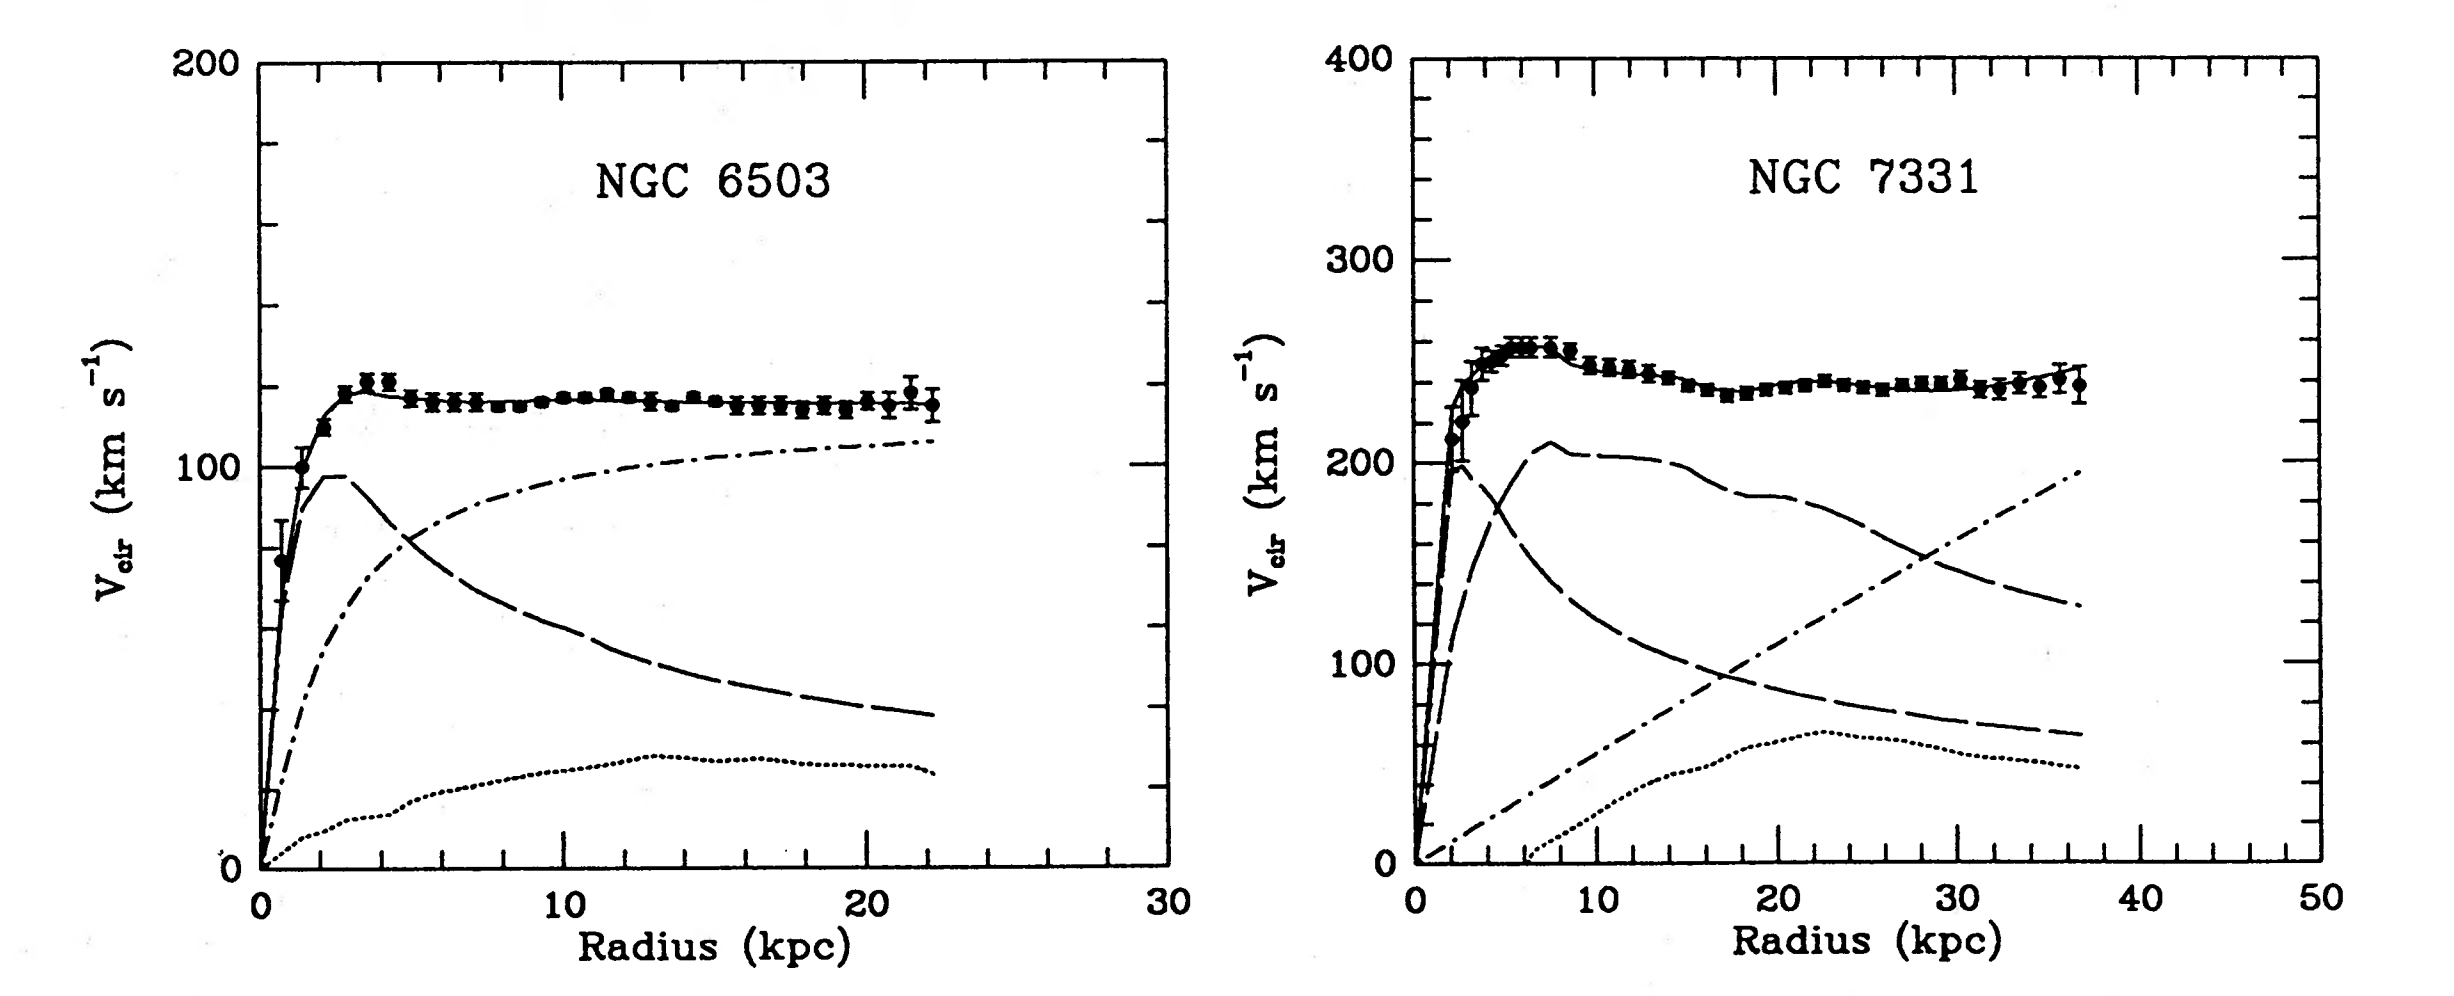
\includegraphics[width=0.85\textwidth]{Motivation/Figures/rotation_curves.png}
  \caption{
    The observed (points) and fitted (solid line) rotation curves for two sample galaxies.
    The fit consists of three components: the stellar component (dashed), the interstellar gas (dotted), and the dark matter halo (dash-dotted).
    Reprinted from Reference~\cite{}. % http://adsabs.harvard.edu/abs/1991MNRAS.249..523B
  }
  \label{fig:rotation_curves}
\end{figure}

As a consequence of Einstein's equivalence principle, a massive body will deflect light, a phenomenon know as gravitational lensing.
In the language of general relativity, this means that the photons take the path given by the geodesic lines following the curvature of space-time due to the massive body.
For most observations of gravitational lensing due to astrophysical bodies, the physical size of the lensing object is much smaller than the distance between observer, lens, and source allowing us to use the thin lens approximation.
Approximating the lens as a planar distribution of matter, the angular deflection is given by 
\begin{equation}
  \vec \alpha (\vec x) = \frac{4G}{c^2} \int \text{d}^2 x' \frac{\vec x - \vec {x'}}{\abs{\vec x - \vec{x'}}^2} 
  \int \text{d} z \rho(\vec{x'}, z)
\end{equation}
where $\vec x$ is a two-dimensional vector in the plane of the lens, $z$ is the perpendicular distance from the plane of the lens, and  $\rho$ is the three dimensional density.
If the source is treated as a point mass, this reduces to
\begin{equation}
  \alpha = \frac{ 4 G} {c^2} \cdot \frac{M}{b}
\end{equation}
where $b = \abs{\vec x - \vec{x'}}$ is the impact parameter and $M$ is the total mass of the object.
% The angle of deflection from the path traveled in the absence of a deflecting body is directly proportional to the mass of the deflecting body.
Thus, measuring the angle of deflection due to gravitional lensing around an astrophysical object provides an independent measurement of the total mass of the body which can be compared against the mass of the luminous objects in the body.
% https://arxiv.org/pdf/1001.1739.pdf

\begin{figure}[htbp]
  \centering
  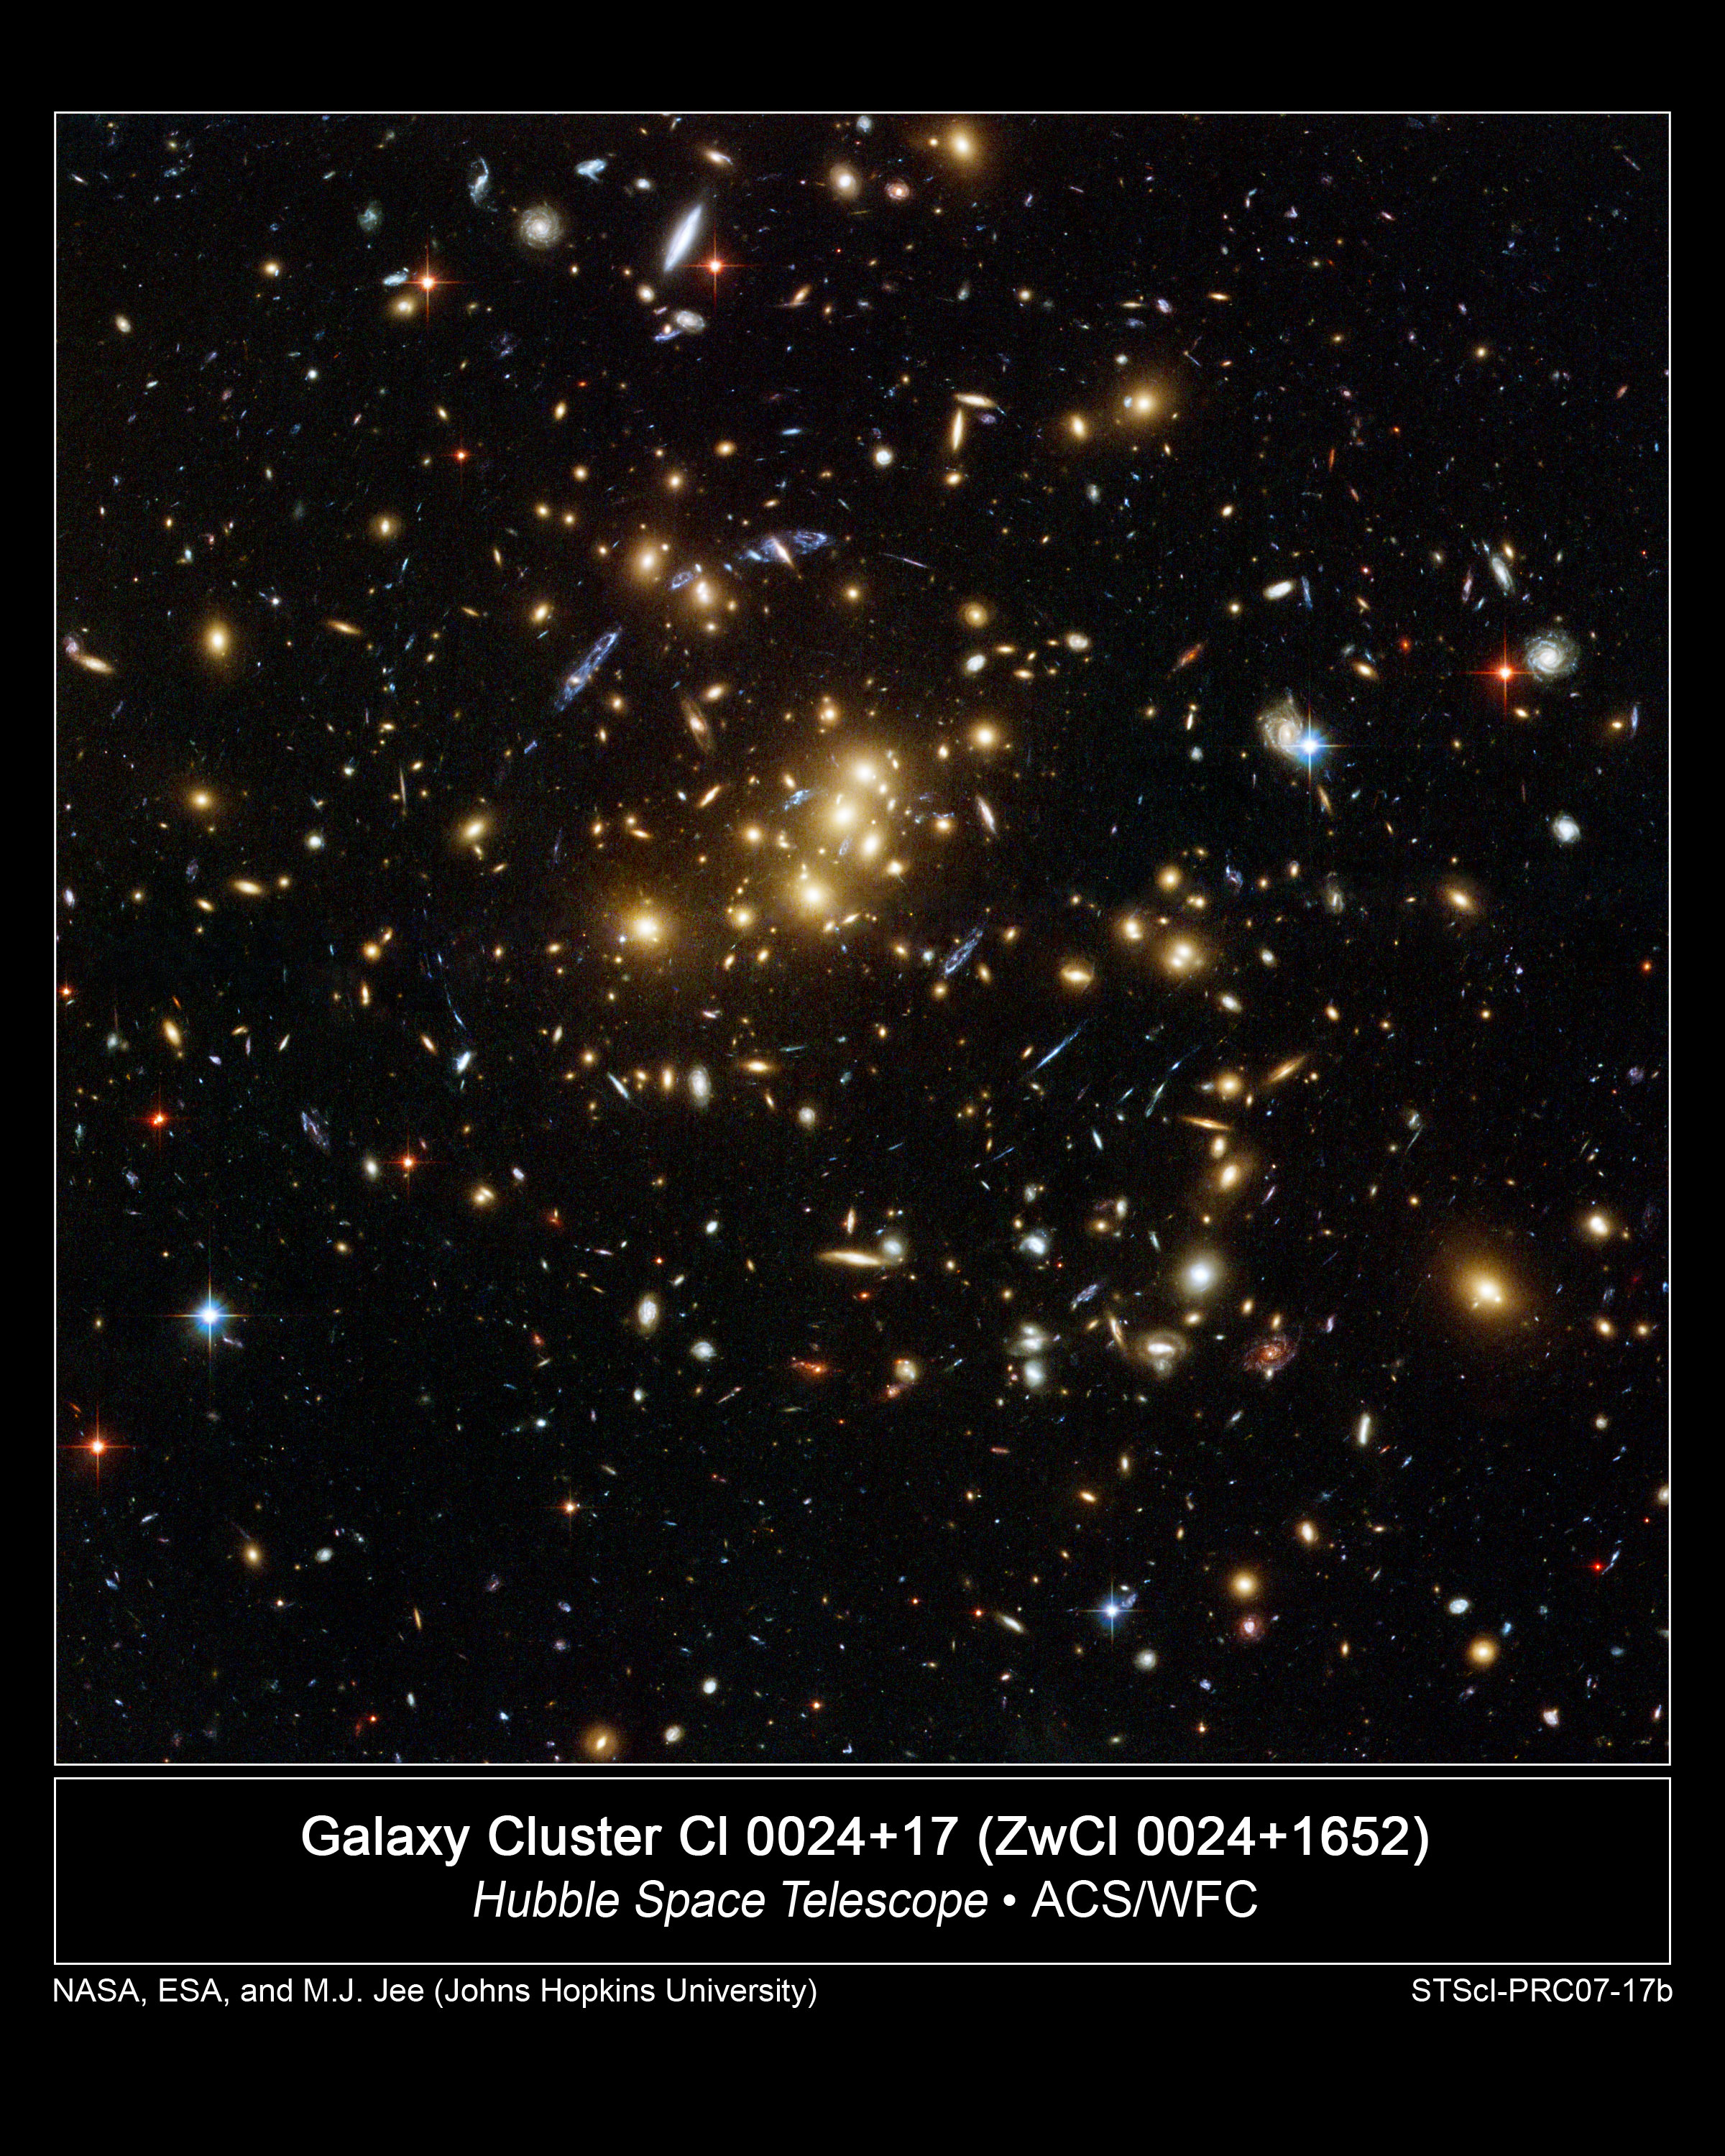
\includegraphics[width=\textwidth]{Motivation/Figures/strong_lensing.jpg}
  \caption{
    Strong gravitational lensing around galaxy cluster CL0024+17, consisting of the graviationally bound yellow, elliptical galaxies.
    The elongated blue objects are from much more distant galaxies behind the cluster which are distorted into arcs due to gravitational lensing from the dark matter halo surrounding the cluster.
    Figure credit:  NASA, ESA, M.J. Jee and H. Ford (Johns Hopkins University)
  }
  \label{fig:strong_lensing}
\end{figure}

Depending on the mass of the deflecting body and impact parameter, the size of deflection can fall into three different regimes.
The first of these is called strong lensing where the curving of space-time is so strong that light can travel multiple paths around the lens and still reach the observer.
If the source is directly behind a circular lens, light travels around all sides of the lens and appears as an Einstein ring, while if the source is offset or the lens is non-circular, the source will instead appear in multiple locations as if viewed from slightly different angles.
An example of strong lensing is shown in Figure~\ref{fig:strong_lensing}.

\begin{figure}[htbp]
  \centering
  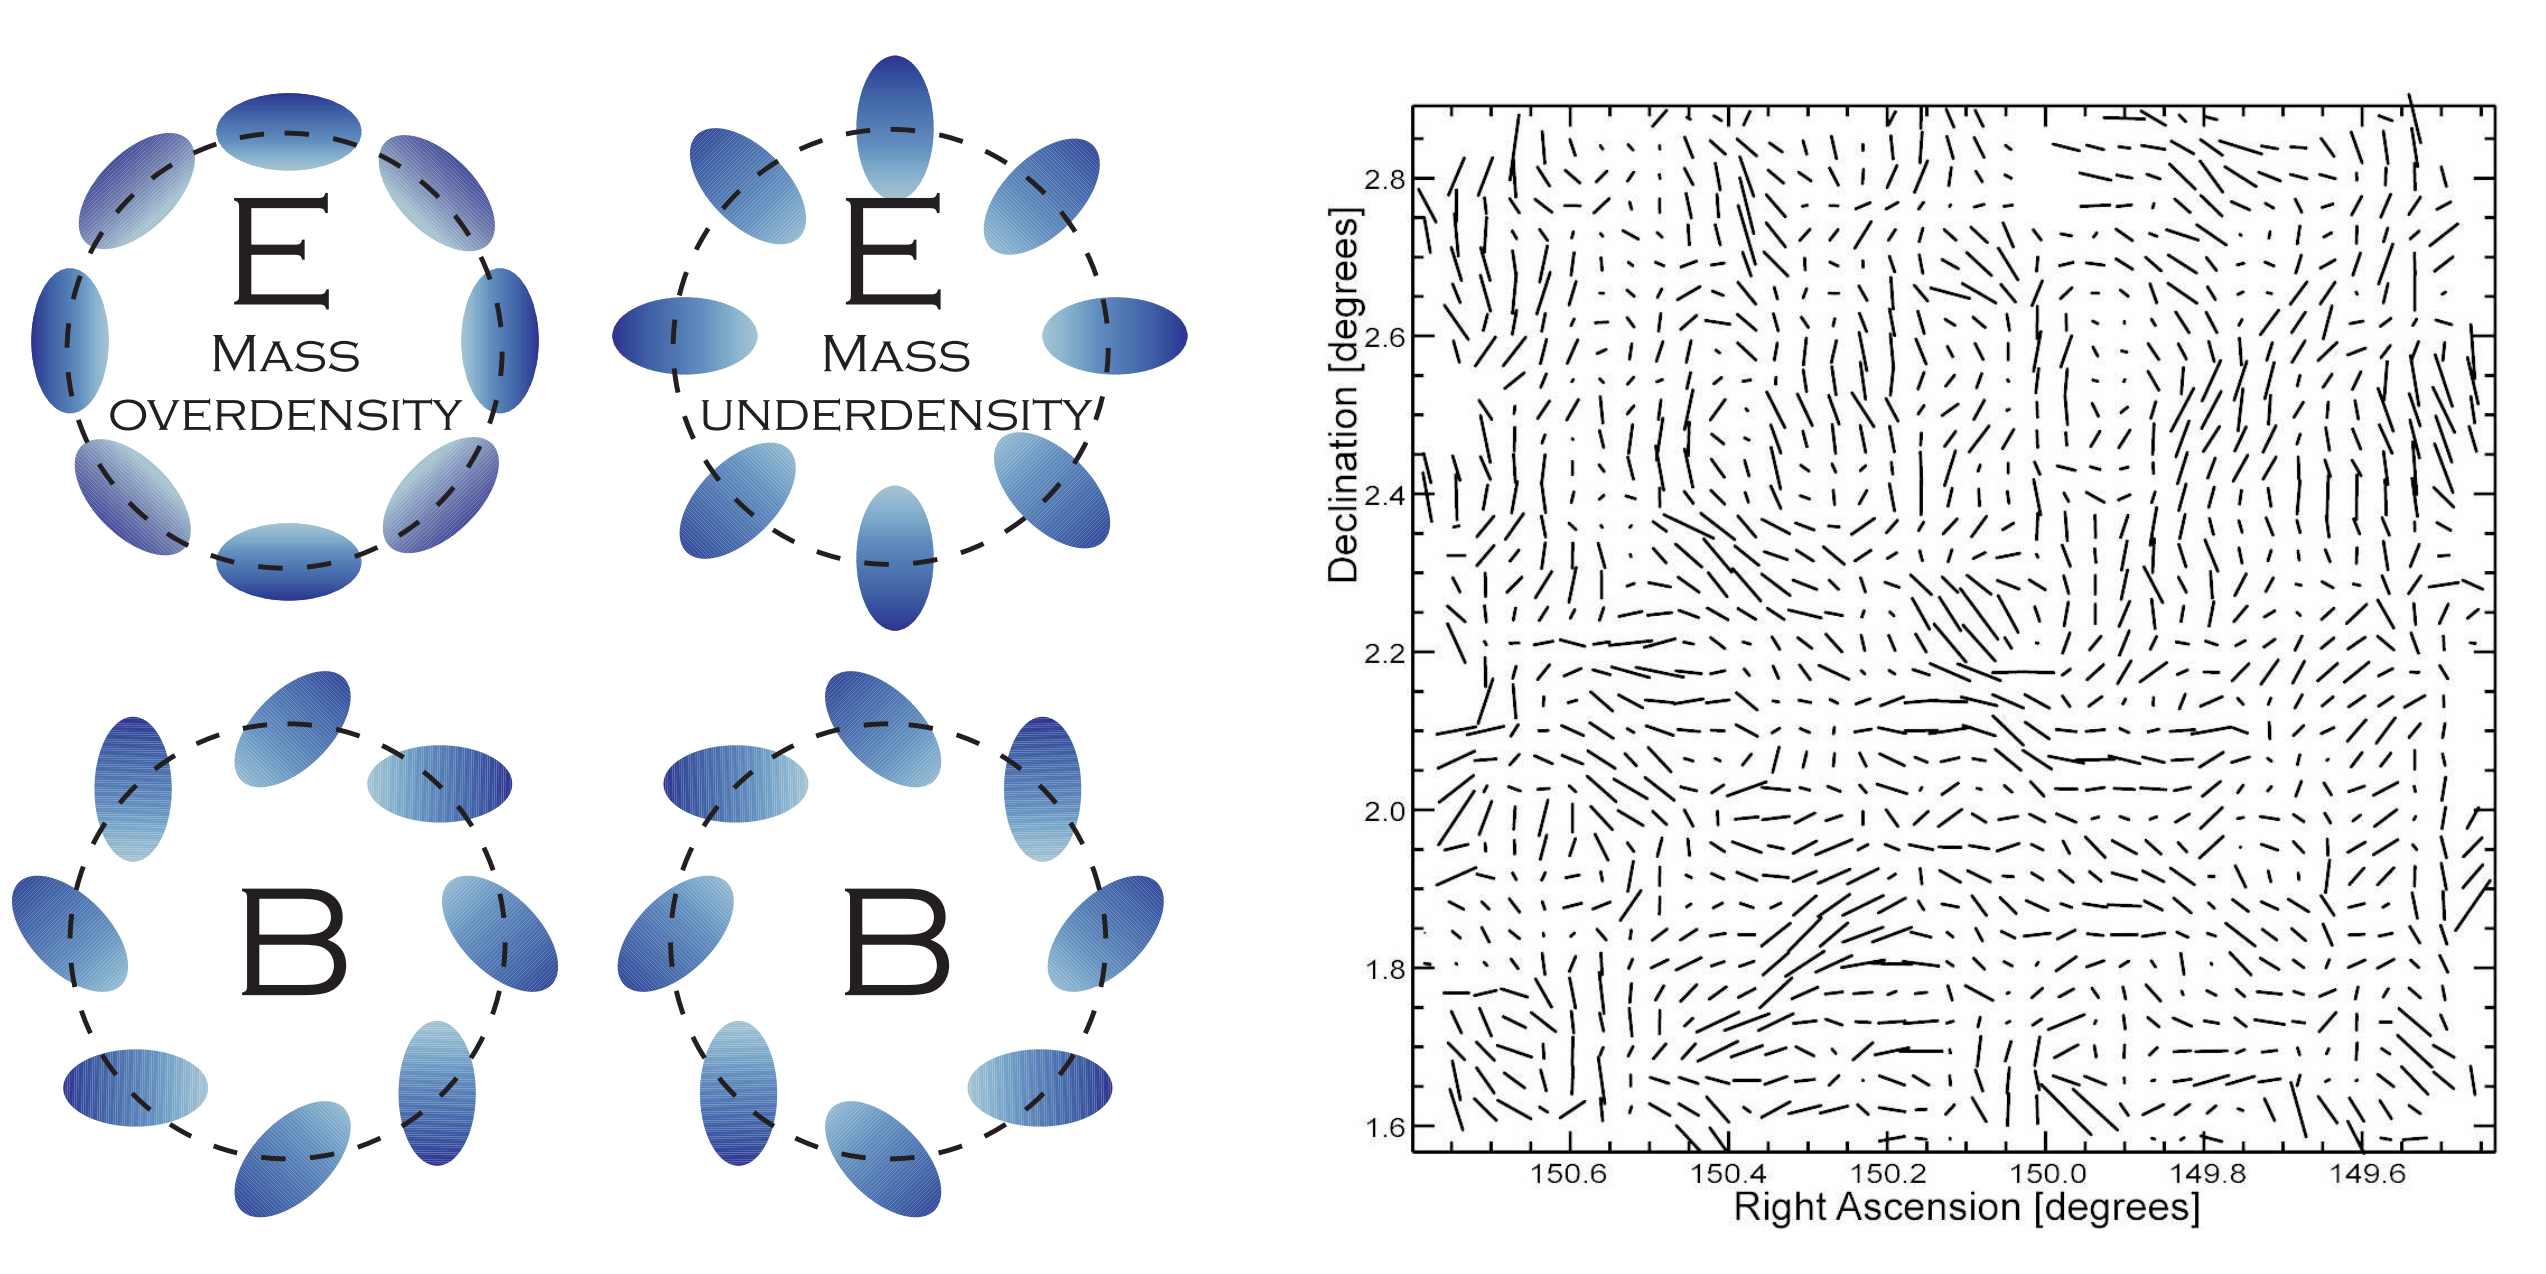
\includegraphics[width=\textwidth]{Motivation/Figures/weak_lensing.png}
  \caption{
    Left: Examples of circular ``$E$-mode'' and curl-like ``$B$-mode'' patterns.
    Right: The observed ellipticities of half a million distant galaxies within the 2 square degree Hubble Space Telescope COSMOS survey.
    Reprinted fom Reference~\cite{}. % https://arxiv.org/abs/1001.1739
  }
  \label{fig:weak_lensing}
\end{figure}

The next regime is known as weak lensing, where the deflection is enough to distort the image of the source but not enough to result in multiple images.
The shear of this distortion can be converted into a map of the projected mass distribution.
True weak lensing results in circular ``$E$-mode'' patterns while sources of systematic uncertainty produce ``$E$-mode'' and curl-like ``$B$-mode'' patterns.
Thus, requiring a zero ``$B$-mode'' contribution assures that the measured mass distribution is accurate.
Figure~\ref{fig:weak_lensing} shows the observed shear of half a million galaxies measured in the Hubble Space Telescope COSMOS survey.

The final regime is the micolensing that occurs when a lens moves relative to a luminous source.
As the lens passes in front of the source, it will temporarily increase the apparent luminosity of the source, enabling a mass measurement of the lens.
Microlensing results show that rocky exoplanets orbit other stars and that these planets cannot form the bulk of dark matter in the Milky Way.

\begin{figure}[htbp]
  \centering
  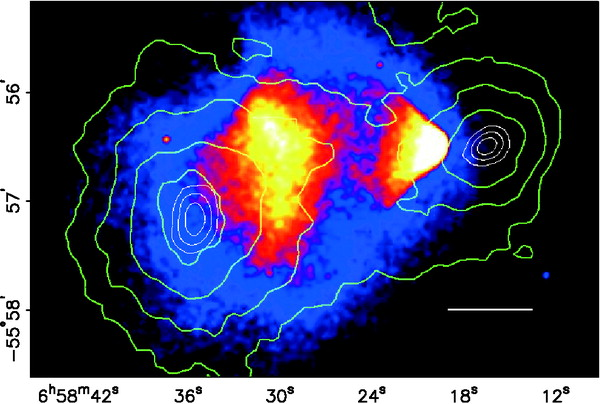
\includegraphics[width=0.75\textwidth]{Motivation/Figures/bullet_cluster.jpg}
  \caption{
    The merging cluster 1E0657-558.
    The green contours show the weak lensing reconstruction of the gravitational potential of the cluster.
    The colors indicate the X-ray temperature of the plasma, changing from blue to white as the plasma goes from coolest to hottest.
    The smaller ``bullet'' cluster on the right which traversed through the larger cluster on the left.
    Reprinted from Reference~\cite{}. % https://iopscience.iop.org/article/10.1086/508162
  }
  \label{fig:bullet_cluster}
\end{figure}

Additionally, gravitational lensing measurements of galactic cluster collisions provide support for dark matter and help constrain its properties.
Figure~\ref{fig:bullet_cluster} shows the merging cluster 1E0657-558.
By comparing the weak lensing reconstruction of the gravitational potential of the cluster shown in green contours against temperature color gradient of the X-ray emitting interstellar plasma, it was learned that the gravitational potential of the cluster doesn't track the dominant baryonic mass contribution coming from the plasma.
Instead, the gravitational potential tracks the smaller stellar baryonic mass component.
Dark matter must be the dominant gravitational source in the cluster since the center of total mass is offset from the center of baryonic mass.
Furthermore, the observation of two gravitional mass centers places strong constraints on the self-interaction of dark matter requiring that the observed mass must have a self-interaction collisional cross section $\sigma/m < 1.25\cm^2\text{g}^{-1}$ at a 68\% confidence level.

\subsection{Relic Density}
\label{sec:dm_relic}

Gonna do some calculations.

At thermal equilibrium, the number density of dark matter $\chi$ is given by
\begin{equation}
  n_\chi^{\text{eq}} = \frac{g}{(2\pi)^3} \int f(\vec p) \, \text{d}^3 \vec p,
\end{equation}
where $g$ is the number of internal degrees of freedom of the particle and $f(\vec p)$ is either the Fermi-Dirac or Bose-Einstein distribution.
The time evolution of the number density $n_\chi (t)$ of dark matter is given by
\begin{equation}
  \frac{\text{d} n_\chi}{\text{d}t} + 3 H n_\chi = - \langle \sigma_A v \rangle \left[ (n_\chi)^2 - (n_\chi^{\text{eq}})^2\right],
\end{equation}
where $H$ is the Hubble expansion rate and $\langle \sigma_A v \rangle$ is the thermally averaged product of the total cross section for annihilation $\sigma_A$ and the  relative velocity $v$ of the dark matter particles.
A dimensional approximation of the present mass density of dark matter is
\begin{equation}
  \Omega_\chi \cdot h^2 = \frac{m_\chi n_\chi}{\rho_c} \simeq \frac{3 \times 10^{-27} \cm^{3} s^{-1}}{\langle \sigma_A v \rangle},
\end{equation}
where $m_\chi$ is the mass of the dark matter particle and $\rho_c = 3H^2/(8\pi G)$ is the critical density of the universe.

\begin{figure}[htbp]
  \centering
  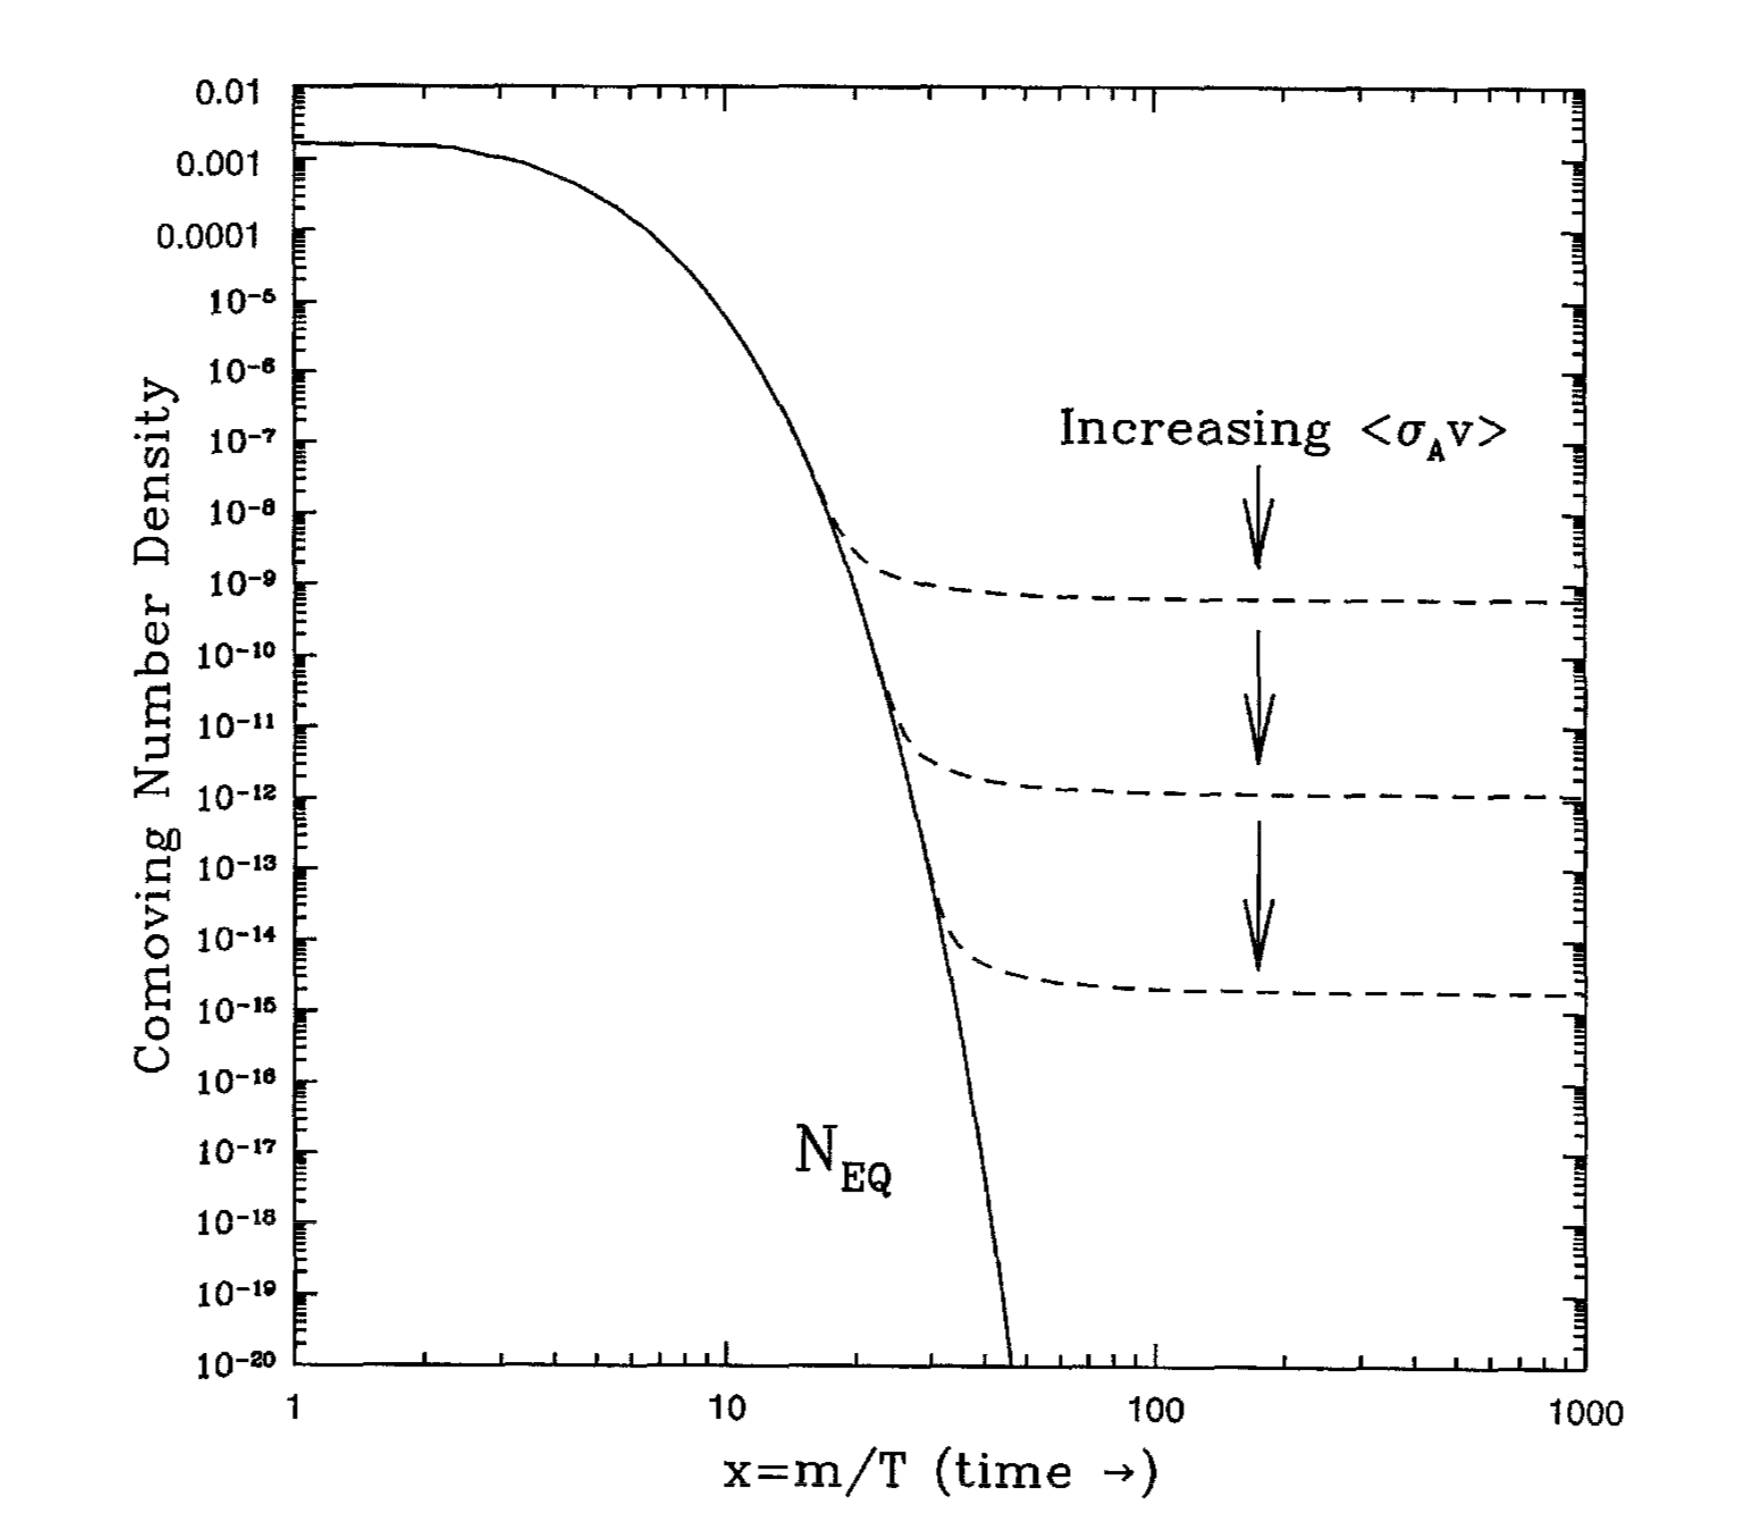
\includegraphics[width=0.625\textwidth]{Motivation/Figures/relic_density.png}
  \caption{
    Relic density of dark matter in the early universe as a function of time.
    The solid curves are the equilibrium abundance while the dashed curves are the actual abundance after freeze-out.
    As the annihilation cross section increases, the relic abundance decreases as the dark matter particles stay in equilibrium longer.
    Reprinted from Reference~\cite{}. % https://doi.org/10.1016/0370-1573(95)00058-5
  }
  \label{fig:relic_density}
\end{figure}

\subsection{Dark Matter Candidates}
\label{sec:dm_cand}

WIMPs, axions, and sterile neutrinos.

\subsection{Non-collider Searches}
\label{sec:dm_search}

Describes.

\subsection{Simplified Models for LHC}
\label{sec:dm_simp}

It was the hot thing at the time.
